
\chapter{Szenen}
\label{Szenen}

Im vorliegenen Projekt wurde für jede Parameterkurve eine eigene Szene erstellt, damit die einzelnen Kurven gegeneinander abgegrenzt sind.

\section{Elemente der Szenen}

\subsection{Prefabs}

\begin{figure}[h!]
	\centering
	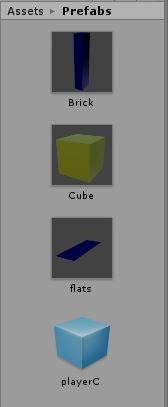
\includegraphics[scale=1]{bilder/prefabs.jpg}
	\caption{Im Projekt verwendete Prefabs}
\end{figure}

Prefabs - PreFabricates, sind bereits vorgefertigte Objekte, die Instanziiert werden müssen. Dies kann auf verschiedenen Wegen geschehen, in diesem Projekt wurden die Prefabs im Unity Editor erzeugt und per Script instantiiert.


\subsection{Scripts}

\subsubsection{Instantiate.cs}
\label{Instantiate}
Dieses Script dient dazu, den Kreis und die PlayerC Punkte zu erzeugen. In der Awake()-Methode werden mittels einer For-Schleife
die Bricks und die PLayerC Objekte erzeugt. Die Plane wird anhand ihres Namens \glqq Boden{}\grqq{} gesucht. Relativ zum Boden wird die Y - Höhe der Bricks berechnet.
Zusätzlich werden die Positionen der einzelnen PlayerC in ein Array geschrieben, dies dient der späteren Pfadanimation.
Es befinden sich noch zwei weitere Funktionen im Script. Diese werden bei jedem Brick bzw. PlayerC aufgerufen. Die X-Koordinate einer Paramterkurve wird über die Funktion $ f(t) = \cos(2 * \pi * t) $ definiert. Für Z gilt $g(t) = \sin(2 * \pi * t)$ analog. Das Parameterintervall ist [0,1]. In diesem Koordinatensystem beschreibt Y die Hochachse.

\textbf{Instantiate\_Spiral.cs}
\label{InstantiateSpiral}

Dieses Script dient dazu, die Spirale und die PlayerC Punkte zu erzeugen. In der Awake()-Methode werden mittels einer For-Schleife die Bricks und die PLayerC Objekte erzeugt. Die Plane wird anhand ihres Namens \glqq Boden{}\grqq{} gesucht. Relativ zum Boden wird die Y - Höhe der Bricks berechnet. Dies geschieht analog zum Kreis.

Ein Vector3-Array wird mit den Koordinaten der PlayerC Objekte gefüllt, damit die Pfadanimation darüber durchgeführt werden kann.

Es befinden sich noch zwei weitere Funktionen im Script. Diese werden bei jedem Brick bzw. PlayerC aufgerufen. Die X.Koordinate einer Paramterkurve wird über die Funktion $ f(t) = t * \cos(2 \pi t) $ definiert. Für Z gilt $g(t) = t * \sin(2 \pi t)$ analog. Das Parameterintervall ist [0,1]. 
\todo{Hier auch noch die 360 punkte erklären} In diesem Koordinatensystem beschreibt Y die Hochachse.
Die Rückgabewerte der Funktionen $f$ und $g$ sind auf 10\% skaliert, damit die Spirale in den Bereich der Plane passt.

\textbf{Instantiate\_Curve.cs}

Dieses Script dient dazu, den Graphen und die PlayerC Punkte zu erzeugen. In der Awake()-Methode werden diese mittels einer For-Schleife erzeugt. 

Die Funktionen für $f$ und $g$ sind ebenfalls im Script. Diese werden bei jedem Brick bzw. PlayerC aufgerufen. Die X - Koordinate einer Parameterkurve wird über die Funktion $ f(t) = t^{2} $ definiert. Für Z gilt $g(t) = t^{3} - 3t$ analog. 


\textbf{Movement.cs}
Dieses Script bewegt den Spieler auf dem Pfad. Dazu werden das Player-GameObject und alle waypoints in der Szene gesucht und adressierbar gemacht.
Wenn die Liste nicht leer ist, dann wird der Spieler und dessen Ziel auf das erste PlayerC gesetzt. 
\emph{Hinweis: Wenn die Liste leer ist, dann kommt es zu einer NullPointer Exception. Jedoch stürzt die Entwicklungsumgebung nicht ab, sondern sie verahrrt im Pause-Modus.}

In der FixedUpdate()-Methode wird nun die Sicht des Spielers auf den nächsten Wegpunkt ausgerichtet. Danach wird der Spieler auf dieses Ziel zubewegt. Sobald der Spieler eine Mindestdistanz zu einem Wegpunkt unterschreitet, wird der Wegpunkt inkrementiert und der Spieler weiter bewegt.

\textbf{CameraController.cs}
Der CamerController sorgt dafür, das die Kamera (in diesem Fall das SteamVR Camera Rig) an der Capsule haftet. Beim Instanzieren, wird der Spieler über den Tag \glqq Player\grqq{} angesprochen und die Position der Camera auf die Position des Spielers gesetzt. 

Um eine Isometrische oder Third-Person-View zu erzeugen müsste die Kamera einen Offset zur Position des Spielers haben. Dies hat sich im hier vorliegenden Kontext als nicht zweckmäßig erwiesen. 

\textbf{SteamVR Scripts}
Das SteamVR Plugin bietet bereits fertige Scripte zur Nutzung der Controller. In dieser Scene werden \emph{SteamVR\_Tracked\_Controller} und \emph{SteamVR\_Laserpointer}. 


\textbf{GraphScene.cs}
Dieses Script ist dem Button, der zur Szene mit der Semikubischen Parabel führt angehängt. Es ruft den SceneManager von Unity auf und übergibt die gewünschte Szene an die Anwendung.

\textbf{SpiralScene.cs}
Dieses Script ist dem Button, der zur Szene mit der Spirale führt angehängt. Es ruft den SceneManager von Unity auf und übergibt die gewünschte Szene an die Anwendung.


\section{Circle}
\label{Kreis}

\begin{figure}[h!]
	\includegraphics[scale=0.5]{bilder/CircleScene.png}
	\caption{Ansicht Circle Scene}
\end{figure}


Die Szene enthält den einen Kreis, der beim Start erzeugt wird. Dieser wird mit konstanter Geschwindigkeit umlaufen. Der Kreis ist mit kleinen Pfosten markiert, die eine Gasse bilden, durch die sich der Spieler automatisch bewegt.



\subsection{3-D Elemente}

\textbf{Plane: } Die Grundfläche der Szene ist eine 4,5 x 3,5 Meter großes 3D-Objekt vom Typ \emph{Plane}.

\textbf{Capsule: } Der Spieler wird mit Hilfe eines GameObjects in Form einer Capsule repräsentiert. Das Camera Rig ist mit Hilfe eines Scripts an dieses Objekt gebunden. Die Capsule hat die Markierung: Player.

\textbf{Brick: } Bricks sind Prefabs, die zur Laufzeit erzeugt werden. Ein einzelner Brick ist konfiguriert, ein Script instanziert Kopien davon.

\textbf{PlayerC: } PlayerC Objekte liegen ebenfalls als Prefab vor. Sie werden in Abhängigkeit der Bricks erzeugt und beschreiben die Positionen, die während der Pfadanimation verwendet werden. PlayerC sind auch GameObjects, haben aber keinen Mesh-Renderer also sind sie unsichtbar. Sie sind als "waypoint" getagged.

\textbf{Canvas: } Auf der Canvas befinden sich zwei Buttons, die dem Szenenwechsel dienen. Die Canvas befindet sich in der Mitte des Kreises. Zur Auswahl einer anderen Szene mit dem Laserpointer des linken Controllers auf den Button zeigen und das Touchpad des Controllers klicken. 


\subsection{Scripte}
\label{Circle_Scripts}
\begin{itemize}
	\item \nameref{Instantiate}, dient der Erzeugung von Steinen und den PlayerC Objekten.
\end{itemize}


\section{Spiral}
\label{Spirale}

\begin{figure}[h!]
	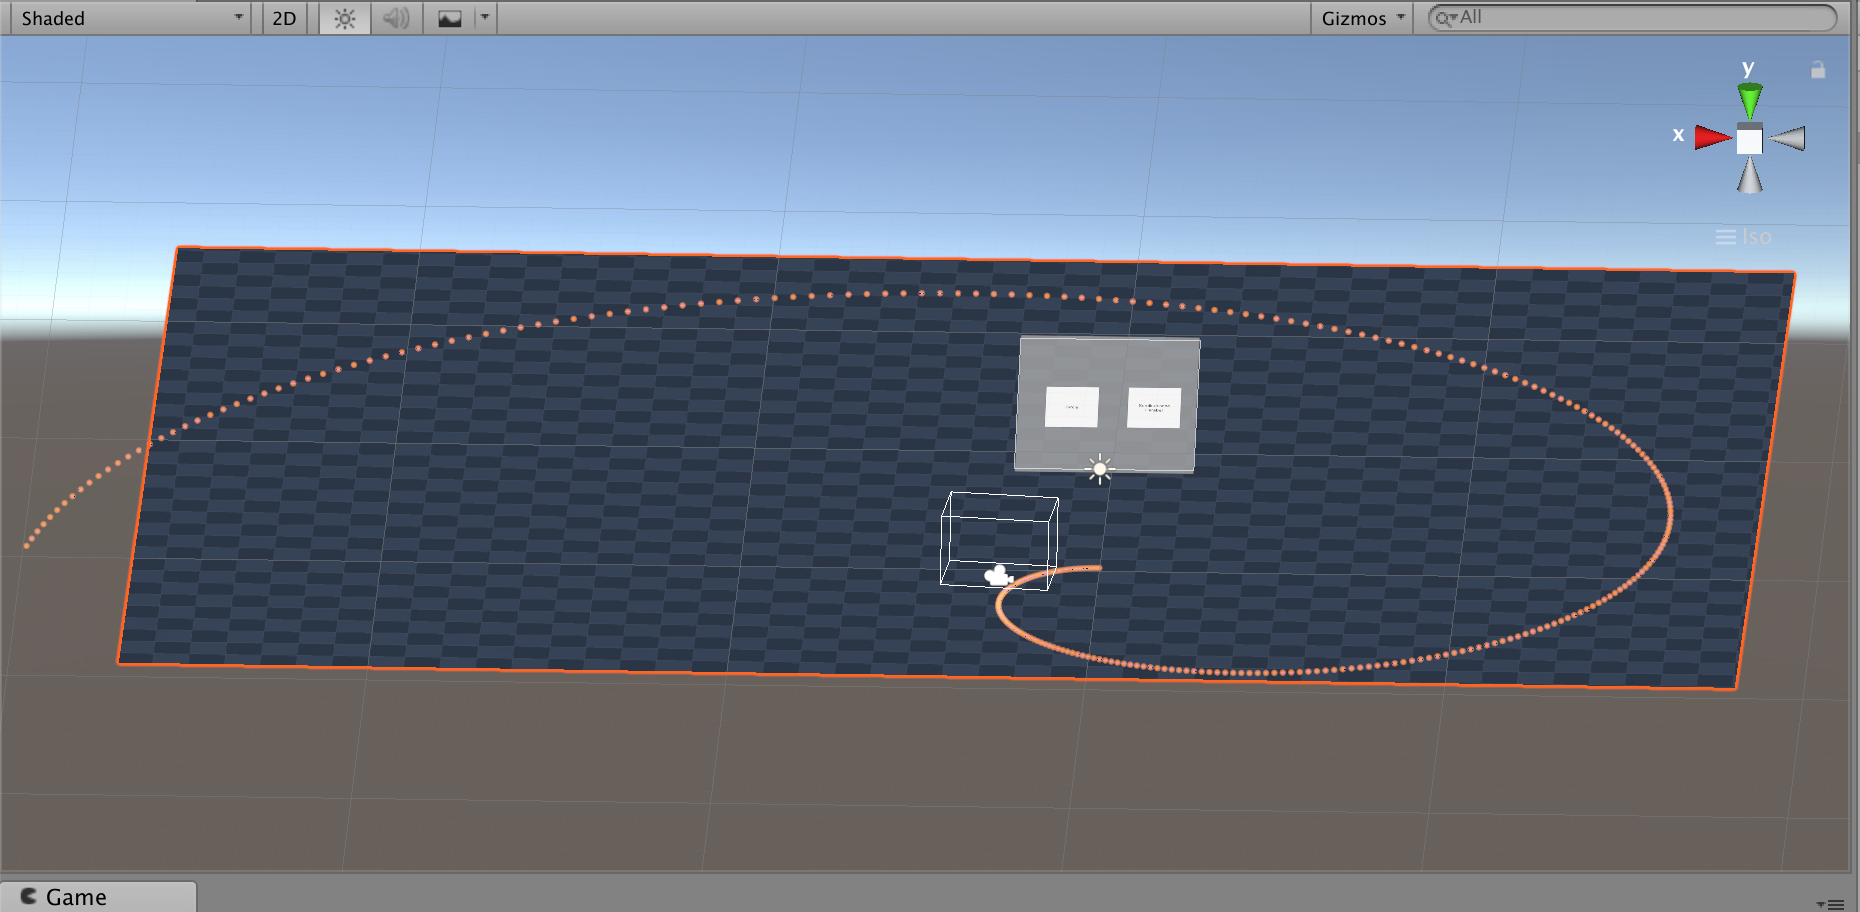
\includegraphics[scale=0.5]{bilder/spiralScene.png}
	\caption{Ansicht Spiral Scene}
\end{figure}


Die Szene enthält den eine Spirale, die beim Start erzeugt wird. Diese wird mit konstanter Geschindigkeit abgefahren. Die Spirale ist mit leuchtenden Quadraten auf dem Boden markiert. Bei Erreichen der letzten Koordinate bewegt sich der Spieler wieder in Richtung des Startpunktes. 

\subsection{3D - Elemente}

\textbf{Plane: } Die Grundfläche der Szene ist eine rotierte 4,5 x 3,5 Meter großes 3D-Objekt vom Typ \emph{Plane}.

\textbf{Capsule: } Der Spieler wird mit Hilfe eines GameObjects in Form einer Capsule repräsentiert. Das Camera Rig ist mit Hilfe eines Scripts an dieses Objekt gebunden. Die Capsule hat die Markierung: Player.

\textbf{Brick: } Bricks sind Prefabs, die zur Laufzeit erzeugt werden. Ein einzelner Brick ist konfiguriert, ein Script instanziert Kopien davon.

\textbf{PlayerC: } PlayerC Objekte liegen ebenfalls als Prefab vor. Sie werden in Abhängigkeit der Bricks erzeugt und beschreiben die Positionen, die während der Pfadanimation verwendet werden. PlayerC sind auch GameObjects, haben aber keinen Mesh-Renderer also sind sie unsichtbar. Sie sind als "waypoint" getagged.

\textbf{Canvas: } Auf der Canvas befinden sich zwei Buttons, die dem Szenenwechsel dienen. Die Canvas befindet sich in der Mitte des Kreises. Zur Auswahl einer anderen Szene mit dem Laserpointer des linken Controllers auf den Button zeigen und das Touchpad des Controllers klicken. 

\subsection{Scripts}
\textbf{Instantiate\_Spiral.cs}
\todo{Spirale Beschreiben}
Dieses Script dient dazu, die Spirale und die PlayerC Punkte zu erzeugen. In der Awake()-Methode werden mittels einer For-Schleife die Bricks und die PLayerC Objekte erzeugt. Die Plane wird anhand ihres Namens \glqq Boden{}\grqq{} gesucht. Relativ zum Boden wird die Y - Höhe der Bricks berechnet. Dies geschieht analog zum Kreis.

Ein Vector3-Array wird mit den Koordinaten der PlayerC Objekte gefüllt, damit die Pfadanimation darüber durchgeführt werden kann.

Es befinden sich noch zwei weitere Funktionen im Script. Diese werden bei jedem Brick bzw. PlayerC aufgerufen. Die X.Koordinate einer Paramterkurve wird über die Funktion $ f(t) = t * \cos(2 \pi t) $ definiert. Für Z gilt $g(t) = t * \sin(2 \pi t)$ analog. Das Parameterintervall ist [0,1]. 
\todo{Hier auch noch die 360 punkte erklären} In diesem Koordinatensystem beschreibt Y die Hochachse.
Die Rückgabewerte der Funktionen $f$ und $g$ sind auf 10\% skaliert, damit die Spirale in den Bereich der Plane passt.

\section{Graph}
\label{ graphScene }

\begin{figure}[h!]
	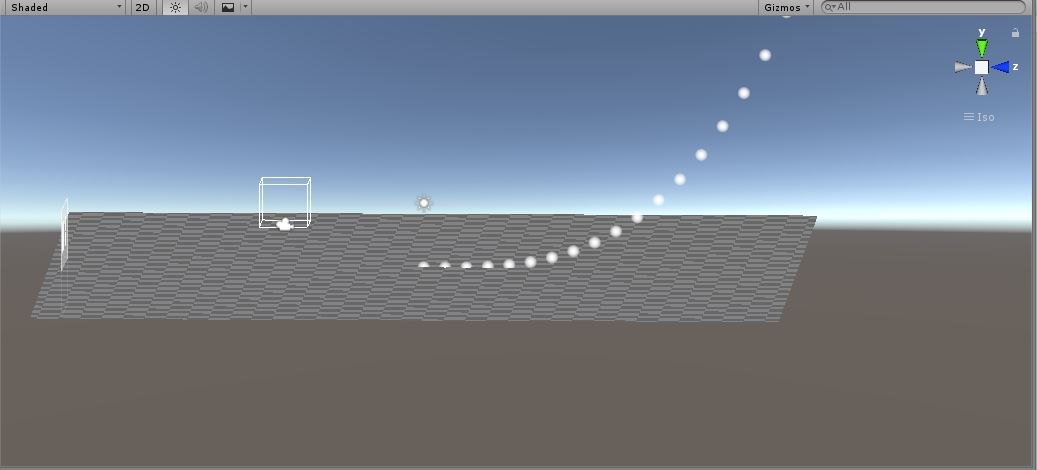
\includegraphics[scale=0.85]{bilder/graphScene.jpg}
	\caption{Ansicht Graph Scene}
\end{figure}

Die Szene enthält den ein Graphen, der beim Start erzeugt wird. Der Graph wird durch leuchtende Würfel dargestellt und ersteckt sich von (0,0,0) in \glqq den Himmel\grqq{}.

Eine Besonderheit dieser Szene ist die Bewegung des Spielers. Im Gegensatz zu den anderen beiden Szenen ist es dem Spieler überlassen, einen geeigneten Standort für die Betrachtung des Graphen zu wählen. Dies geschieht über Teleportation. 

Mit dem linken Controller, der einen Laserstrahl emittiert wird das Ziel gewählt und mit einem Druck auf den Trigger wird ein Teleport ausgelöst. 

\todo{Mglw Fahrstuhl einbauen} 

\subsection{3D - Elemente}

\textbf{Plane: } Die Grundfläche der Szene ist eine rotierte 4,5 x 3,5 Meter großes 3D-Objekt vom Typ \emph{Plane}.

\textbf{Capsule: } Der Spieler wird mit Hilfe eines GameObjects in Form einer Capsule repräsentiert. Das Camera Rig ist mit Hilfe eines Scripts an dieses Objekt gebunden. Die Capsule hat die Markierung: Player.

\textbf{Cube: } Cubes sind Prefabs, die zur Laufzeit erzeugt werden. Ein einzelner Cube ist konfiguriert, ein Script instanziert Kopien davon.

\textbf{PlayerC: } PlayerC Objekte liegen ebenfalls als Prefab vor. Sie werden in Abhängigkeit der Bricks erzeugt und beschreiben die Positionen, die während der Pfadanimation verwendet werden. PlayerC sind auch GameObjects, besitzen aber keinen Mesh-Renderer also sind sie unsichtbar. PlayerC Prefabs sind als "waypoint" getagged.

\textbf{Canvas: } Auf der Canvas befinden sich zwei Buttons, die dem Szenenwechsel dienen. Die Canvas befindet sich in der Mitte des Kreises. Zur Auswahl einer anderen Szene mit dem Laserpointer des linken Controllers auf den Button zeigen und das Touchpad des Controllers klicken. 

\subsection{Scripts}
\textbf{Instantiate\_Curve.cs}

Dieses Script dient dazu, den Graphen und die PlayerC Punkte zu erzeugen. In der Awake()-Methode werden diese mittels einer For-Schleife erzeugt. 

Die Funktionen für $f$ und $g$ sind ebenfalls im Script. Diese werden bei jedem Brick bzw. PlayerC aufgerufen. Die X - Koordinate einer Parameterkurve wird über die Funktion $ f(t) = t^{2} $ definiert. Für Z gilt $g(t) = t^{3} - 3t$ analog. 



